% =============================================================================
%  Sección 0: Introducción
%  Sustituye el contenido de \lipsum con tu propio texto.
% =============================================================================

\section{Introducción}
\label{sec:introduccion}
Durante la década de 1930, México se encontraba en un proceso de consolidación política 
tras el conflicto revolucionario iniciado en 1910. En este periodo de modernización 
nacional impulsado por el general Lázaro Cárdenas, las comunidades rurales del sur del 
Valle de México comenzaron a integrarse formalmente a la estructura del Estado 
posrevolucionario \cite{lopez2017indigenas}.

\subsection{Antecedentes o Contexto Histórico}
\label{sec:antescendetes}

Las primeras décadas del siglo XX en Milpa Alta estuvieron marcadas por su rol 
estratégico como conector entre el estado de Morelos, cuna del zapatismo, y la Ciudad de 
México. Debido a su perfil agrario, el movimiento zapatista representó una 
esperanza de cambio para estos pueblos, albergando incluso el Cuartel Zapatista del Sur
\cite{fundacionunam2020historia}.

Sin embargo, tras sucesos trágicos como la \termino{Matanza de Chapitel} en 1916, 
el poblado de San Pedro Atocpan experimentó un desarrollo lento y complejo. 
La memoria histórica de la región aún conserva el dolor de la guerra revolucionaria, 
el cual se entrelaza con el hito de la \textbf{tromba de 1935}. 
Este evento no solo destruyó la precaria infraestructura existente, sino que marcó un 
punto de inflexión en las dinámicas económicas y en la gestión del territorio hacia la 
mitad del siglo \cite{santuarioSFtesoro}.

\subsection{Origen Étnico y Territorial de Milpa Alta}
\label{sec:origen-etnico}

La demarcación de Milpa Alta posee un carácter predominantemente rural cuyas raíces 
se remontan al año 1429. Según las crónicas locales, el sabio consejero 
\textit{Tlacaelel} ordenó a \textit{Hueyitlahuilanque} comandar la exploración y 
conquista de la región de \textbf{Malacaxtepec Momoxco}. Tras vencer a los grupos 
chichimecas de la zona, se establecieron nuevos caminos y poblados, dando origen a 
asentamientos como \termino{Oztotepec}, \termino{Tlacoyucan} y el calpulli 
\termino{Xaxahuanco}, donde eventualmente surgió Atocpan.

La identidad de estos pueblos está profundamente ligada a su lengua y a la toponimia náhuatl, 
la cual refleja las características geográficas de su emplazamiento. En el Cuadro 
\ref{tab:pueblos_milpa_alta} se detalla el significado de los asentamientos que 
conforman la actual Milpa Alta.

\begin{table}[H]
    \centering
    \caption[Significado de los pueblos originarios de Milpa Alta]
    {Significado de los pueblos originarios de Milpa Alta.}
    \label{tab:pueblos_milpa_alta}
    \fontsize{9pt}{11pt}\selectfont % Ajuste de fuente para acomodar el texto denso
    \begin{tabularx}{\textwidth}{l l X X X}
        \toprule
        \textbf{Nombre actual} & \textbf{Forma en náhuatl} & \textbf{Análisis morfológico} & \textbf{Traducción literal} & \textbf{Significado interpretativo} \\
        \midrule
        Oztotepec & Oztōtēpēc & oztōtl (cueva) + tēpēc (en el cerro, sobre el cerro) & ``En el cerro de las cuevas'' & Lugar montañoso con grutas o cuevas naturales, posiblemente con función ritual o de refugio. \\
        \addlinespace
        Tlacoyucan & Tlācoyōcān & tlācoyōtl (figura alargada) + -cān (lugar de) & ``Lugar de tlacoyos'' o ``Lugar alargado'' & Puede aludir a la forma del terreno o a la producción del alimento tradicional. \\
        \addlinespace
        Tlacotenco & Tlacōtenco & tlacōtl (vara, bastón, caña) + -tenco (a la orilla de) & ``A la orilla de los carrizos'' & Sitio donde crecían cañas o varas junto a un borde o ribera. \\
        \addlinespace
        Tepenahuac & Tēpēnahuac & tēpētl (cerro) + nahuac (junto a, cerca de) & ``Junto al cerro'' & Asentamiento al pie o al costado de un cerro. \\
        \addlinespace
        Tecoxpa / Tecozpa & Tēcōxpan & tēcōxtli (piedra amarilla o miel) + -pan (sobre, en) & ``En la piedra amarilla'' & Lugar con piedra volcánica amarillenta o cantera. \\
        \addlinespace
        Micatlán / Miacatlán & Mīacatlān & mīa (mucho, abundante) + -tlān (lugar de) & ``Lugar abundante'' & Denota fertilidad o abundancia de recursos naturales. \\
        \addlinespace
        Atocpan & Ātōcpan & ātl (agua) + tocpān (sobre el lodo o barro) & ``Sobre el lodo'' o ``Lugar en el agua y el barro'' & Alude a suelos húmedos y fértiles, próximos a zonas lacustres. \\
        \addlinespace
        Ohtenco & Ōhtenco & ōhtli (camino) + -tenco (a la orilla de) & ``A la orilla del camino'' & Lugar ubicado junto a un sendero o vía principal; vinculado a rutas comerciales. \\
        \addlinespace
        Xicomulco & Xīcomōlco & xīcomōlli (jícaro, vasija) + -co (en) & ``En el jícaro'' o ``Lugar de jícaras'' & Sitio donde abundaban los árboles de jícaro o donde se fabricaban vasijas. \\
        \addlinespace
        Tecomitl & Tēcomitl & tēcomitl (cántaro, olla, vasija) & ``El cántaro'' o ``Lugar de cántaros'' & Hace referencia a producción o forma del terreno semejante a una vasija. \\
        \addlinespace
        Malacachtepec & Malacachtepēc & malacach-tli (trenza, cuerda enrollada) + tēpēc (en el cerro) & ``En el cerro de las trenzas'' o ``Lugar del cerro torcido'' & Puede referirse a colinas de forma ondulante o caminos sinuosos. \\
        \addlinespace
        Cuauhtenco & Cuāuhtenco & cuāuhtli (águila o árbol) + -tenco (a la orilla de) & ``A la orilla del árbol / del bosque / del águila'' & Sitio ubicado al borde de un bosque o asociado al símbolo del águila. \\
        \midrule
        \multicolumn{5}{l}{\footnotesize \textit{Fuente:} Elaborado con traducciones propias a partir de \cite{diccionario_nahuatl2018}.} \\
        \bottomrule
    \end{tabularx}
\end{table}

La toponimia de \textit{Atocpan} es particularmente relevante para este plan de regeneración, 
pues alude directamente a suelos húmedos y fértiles, advirtiendo desde su origen la 
relación intrínseca del pueblo con el agua y su vulnerabilidad geográfica \citep{fundacionunam2020historia}, 
tal como se ilustra en la \ref{fig:cuenca_mexico_comparativa}.

% NOTA: Si tu documento es a doble columna, cambia {figure} por {figure*}
\begin{figure}[!ht]
    \centering
    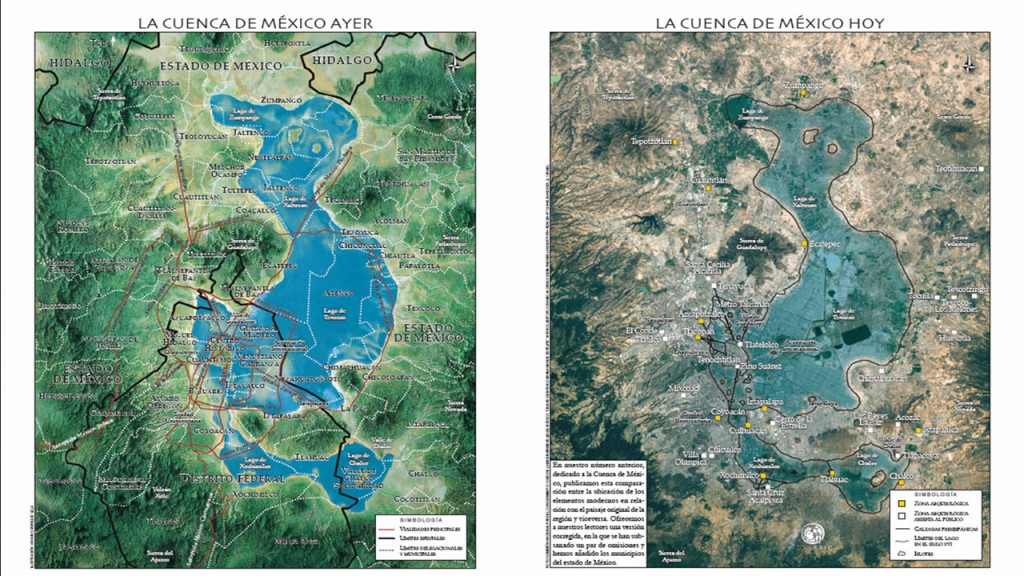
\includegraphics[width=0.95\textwidth]{img/imagenes/CUENCA.jpg}
    \caption{Comparativa histórica de la evolución hidrológica en el Valle de México: 
            La Cuenca de México ayer (izquierda) y hoy (derecha). Adaptado de 
            \cite{fundacionunam2020historia}.}
    \label{fig:cuenca_mexico_comparativa}
\end{figure}
